% v1.7 - 2014-11-18
% - bib fixes: now using biber instead of bibtex (thanks felix)
% - compile now with pdflatex -> biber -> pdflatex
% v1.6 - 2013-05-13
% - bibliography headers fixed - thanx lorenz lehmann
% - high quality titlepage - thanx thomas graf
% - removed separation of online and offline references -> style 1.4a
% v1.5 - 2013-01-16

\documentclass[twoside,11pt,titlepage,a4paper,english,bibliography=totocnumbered,listof=numbered]{scrbook}

% Template Style
% =========================================================================
% = SNET THESIS TEMPLATE STYLE
% =========================================================================

% http://www.snet.tu-berlin.de
% ------------------------
% Adapted version from http://hci.rwth-aachen.de/karrer_thesistemplate (Thorsten Karrer)
% Further adaptions for http://www.elearn.rwth-aachen.de (Sascha Hoellger)
% Further adaptions for SNET @ TU Berlin by Sebastian Göndör (sebastian.goendoer@tu-berlin.de)


% =========================================================================
% = CHANGELOG
% =========================================================================

% [0.1.4b]
% backend=biber added in line 139
% 
% [0.1.4a]
% title page: image logo sizes and margins adjusted to printable area
% removed separation of online and offline references
%
% [0.1.3]
% wider text body
% added "school" to the titlepage
% paragraph indents
% correctly placed footnote graphics
% 
% [0.1.2]
% new titlepage
% some minor fixes
% 
% [0.1.1]
% changed titlepage logo
% added listoffigures and listoftables
% excluded abstract from toc
% no (roman) numbering for frontmatter
% 
% [0.1]
% adapted version 0.991b from sascha hoellger @ rwth aachen


% =========================================================================
% = MISC
% =========================================================================

\usepackage{a4wide}					% 
\usepackage{verbatim}				% 
\usepackage[toc,page]{appendix}			% 
\usepackage[withpage]{acronym}			% 
\usepackage{amsthm}				% Definitions


% =========================================================================
% = COLORS
% =========================================================================

\usepackage{xcolor}					% Colors
\definecolor{LightBlue}{rgb}{0.55,0.55,1}
\definecolor{DarkBlue}{rgb}{0.2,0.2,0.5}
\definecolor{DarkRed}{rgb}{0.71,0.12,0.07}

% =========================================================================
% = PAGE LAYOUT
% =========================================================================

\usepackage{geometry}
\geometry{inner=3cm, outer=2cm, bottom=4cm}

\newcommand{\setwidesite}				% changes the geometry to have less margin
{
	\fancyhfoffset[LE,RO]{0cm}
	\fancyheadoffset[LO,RE]{0cm}
	\fancyfootoffset[RE]{2cm}
	\newgeometry{inner=2cm, outer=2cm, bottom=4cm}
}

\usepackage{noindent}				%do not indent at new paragraphs but add a vertical offset

\setlength{\parindent}{4mm}
\setlength{\parskip}{1.5mm }


% =========================================================================
% = TYPESETTING
% =========================================================================

\usepackage[hyphens]{url}				% url
\usepackage{hyphenat}				% hyphenation. use \hyphenation{}

\righthyphenmin=5
\lefthyphenmin=5


% =========================================================================
% = TABLE OF CONTENTS
% =========================================================================

\setcounter{secnumdepth}{4}
\setcounter{tocdepth}{3} 


% =========================================================================
% = FONTS
% =========================================================================

\usepackage{mathpazo} 
\usepackage[scaled=.95]{helvet} 
\usepackage{courier} 


% =========================================================================
% = SYMBOLS
% =========================================================================

%\usepackage{gensymb}
\usepackage{textcomp} 				% for \textmu (non-italic $\mu$)
\makeatletter						% this makes "@" a regular letter


% =========================================================================
% = TABLES
% =========================================================================

\usepackage{tabularx}
\usepackage{booktabs}
\usepackage{multirow}
\usepackage{longtable}				% tables spanning over more than one page

%%\setlength{\fboxsep}{0mm}			% spacing between \fbox border and content

\usepackage{amsmath}				% math fonts
\usepackage{amssymb}				% math symbols
\usepackage{setspace}				% line spacing 


% =========================================================================
% = BIBIOGRAPHY
% =========================================================================

\usepackage[style=numeric,natbib=true,backend=biber]{biblatex}

% apparently no effect?
%\renewcommand{\bibsetup}{
%	\markboth{
%		\MakeUppercase{Bibliography}
%	}{}
%}

\ifdefined\bibheadingonline
  \defbibheading{online}{\section*{\bibheadingonline}}
\else
  \defbibheading{online}{\section*{Online References}}
\fi
\ifdefined\bibheadingoffline
  \defbibheading{offline}{\section*{\bibheadingoffline}}
\else
  \defbibheading{offline}{\section*{Printed References}}
\fi

\defbibfilter{online}{%
  \( \type{online} \)}

\defbibfilter{offline}{%
  \( \not \type{online} \)}

\bibliography{main}


% =========================================================================
% = LANGUAGE & ENCODING
% =========================================================================

\usepackage[english]{babel}				% \usepackage[ngerman]{babel}

\selectlanguage{english}				% \selectlanguage{ngerman}

\usepackage[T1]{fontenc}
\usepackage[utf8]{inputenc}				% can use native umlauts

% \usepackage[babel,german=quotes]{csquotes}	% provides \enquote{Blupp} => "`Blupp"'
\usepackage[babel,english=american]{csquotes}	% provides \enquote{Blupp} => "`Blupp"'

\SetCiteCommand{\parencite}			% Changed for biblatex

\usepackage{units}					% unified way of setting values with units

\usepackage{appendix}


% =========================================================================
% = CODE LISTINGS
% =========================================================================

\usepackage{listings}

% Listings Styles from Max 

\definecolor{violet}{cmyk}{0.45,0.97,0.27,0.21}
\definecolor{lstblue}{cmyk}{1,0.80,0,0}
\definecolor{lstgreen}{cmyk}{0.71,0.21,0.65,0.22}
\definecolor{bluegrey}{cmyk}{0.56,0.24,0.11,0.05}
\definecolor{javadoc}{cmyk}{0.88,0.59,0,0}
\definecolor{lstgrey}{cmyk}{0.55,0.44,0.42,0.32}

\lstdefinelanguage{SQL}{
     keywords={},
     keywordstyle=\color{bluegrey}\bfseries,
     morekeywords=[2]{CREATE,TABLE,IF,NOT,EXISTS,NULL,SET,DEFAULT,PRIMARY,KEY,COLLATE,CHARACTER,AUTO_INCREMENT,ENGINE,CHARSET},
     keywordstyle={[2]\color{violet}\bfseries},
     otherkeywords={int,varchar,double,text,tinyint},
     sensitive=false,
     morecomment=[l][\color{lstgreen}]{//},
     morecomment=[s][\color{lstgreen}]{/*}{*/},
     morecomment=[s][\color{javadoc}]{/**}{*/},
     morestring=[b]',
     morestring=[b]"
  }
\lstdefinelanguage{PHP}{
     keywords={},
     keywordstyle=\color{bluegrey}\bfseries,
     morekeywords=[2]{static,function,if,return,pow,sin,cos,asin,min,sqrt,int},
     keywordstyle={[2]\color{violet}\bfseries},
     otherkeywords={@param, @returns, @author, @type, @link, @see},
     sensitive=false,
     morecomment=[l][\color{lstgreen}]{//},
     morecomment=[s][\color{lstgreen}]{/*}{*/},
     morecomment=[s][\color{javadoc}]{/**}{*/},
     morestring=[b]',
     morestring=[b]"
  }
\lstdefinelanguage{JavaScript}{
     keywords={},
     keywordstyle=\color{bluegrey}\bfseries,
     morekeywords=[2]{attributes, class, classend, do, empty, endif, endwhile, fail, function, functionend, if, implements, in, inherit, inout, not, of, operations, out, return, set, then, types, while, use},
     keywordstyle={[2]\color{violet}\bfseries},
     otherkeywords={@param, @returns, @author, @type, @link, @see},
     sensitive=false,
     morecomment=[l][\color{lstgreen}]{//},
     morecomment=[s][\color{lstgreen}]{/*}{*/},
     morecomment=[s][\color{javadoc}]{/**}{*/},
     morestring=[b]',
     morestring=[b]"
  }
\lstdefinelanguage{Java}{
     keywords={},
     keywordstyle=\color{bluegrey}\bfseries,
     morekeywords=[2]{abstract,boolean,break,byte,case,catch,char,class,
      const,continue,default,do,double,else,extends,false,final,
      finally,float,for,goto,if,implements,import,instanceof,int,
      interface,label,long,native,new,null,package,private,protected,
      public,return,short,static,super,switch,synchronized,this,throw,
      throws,transient,true,try,void,volatile,while},
     keywordstyle={[2]\color{violet}\bfseries},
     morekeywords=[3]{@SuppressWarnings, @Capability, @Override},
     keywordstyle={[3]\color{lstgrey}},
     otherkeywords={@param, @return, @returns, @author, @link, @see},
     sensitive,
     morecomment=[l]//,
     morecomment=[s]{/*}{*/},
     morecomment=[s][\color{javadoc}]{/**}{*/},
     morestring=[b]",
     morestring=[b]',
  }[keywords,comments,strings]

% some listings styles from Gregor Aisch
% http://vis4.net/blog/2009/09/noch-mehr-sprach-definitionen-fuer-latex-listings/

\lstdefinelanguage{HTML5} {morekeywords={a, abbr, address, area, article, aside, audio, b, base, bb, bdo, blockquote,  body, br, button, canvas, caption, cite, code, col, colgroup, command, datagrid, datalist, dd, del, details, dialog, dfn, div, dl, dt, em, embed, eventsource, fieldset, figure, footer,  form,  h1, h2,  h3,  h4, h5,  h6,  head,  header,  hr, html,  i, iframe,  img,  input,  ins, kbd,  label,  legend,  li,  link,  mark,  map,  menu,  meta,  meter,  nav,  noscript,  object,  ol,  optgroup,  option,  output,  p,  param,  pre,  progress,  q,  ruby,  rp,  rt,  samp,  script,  section,  select,  small,  source,  span,  strong,  style,  sub,  sup,  table,  tbody,  td,  textarea,  tfoot,  th,  thead,  time,  title,  tr,  ul,  var,  video},
sensitive=false, morecomment=[s]{<!--}{-->}, morestring=[b]", morestring=[d]'}

\lstdefinelanguage{CSS} {morekeywords={azimuth,  background-attachment,  background-color,  background-image,  background-position,  background-repeat,  background,  border-collapse,  border-color,  border-spacing,  border-style,  border-top, border-right, border-bottom, border-left,  border-top-color, border-right-color, border-bottom-color, border-left-color,  border-top-style, border-right-style, border-bottom-style, border-left-style,  border-top-width, border-right-width, border-bottom-width, border-left-width,  border-width,  border,  bottom,  caption-side,  clear,  clip,  color,  content,  counter-increment,  counter-reset,  cue-after,  cue-before,  cue,  cursor,  direction,  display,  elevation,  empty-cells,  float,  font-family,  font-size,  font-style,  font-variant,  font-weight,  font,  height,  left,  letter-spacing,  line-height,  list-style-image,  list-style-position,  list-style-type,  list-style,  margin-right, margin-left,  margin-top, margin-bottom,  margin,  max-height,  max-width,  min-height,  min-width,  orphans,  outline-color,  outline-style,  outline-width,  outline,  overflow,  padding-top, padding-right, padding-bottom, padding-left,  padding,  page-break-after,  page-break-before,  page-break-inside,  pause-after,  pause-before,  pause,  pitch-range,  pitch,  play-during,  position,  quotes,  richness,  right,  speak-header,  speak-numeral,  speak-punctuation,  speak,  speech-rate,  stress,  table-layout,  text-align,  text-decoration,  text-indent,  text-transform,  top,  unicode-bidi,  vertical-align,  visibility,  voice-family,  volume,  white-space,  widows,  width,  word-spacing,  z-index},
sensitive=false, morecomment=[s]{/*}{*/}, morestring=[b]", morestring=[d]'}

\lstdefinelanguage{JavaFX} {morekeywords={abstract, after, and, as, assert, at, attribute, before, bind, bound, break, catch, class, continue, def, delete, else, exclusive, extends, false, finally, first, for, from, function, if, import, indexof, in, init, insert, instanceof, into, inverse, last, lazy, mixin, mod, new, not, null, on, or, override, package, postinit, private, protected, public-init, public, public-read, replace, return, reverse, sizeof, static, step, super, then, this, throw, trigger, true, try, tween, typeof, var, where, while, with },
sensitive=false, morecomment=[l]{//}, morecomment=[s]{/*}{*/}, morestring=[b]", morestring=[d]'}

\lstdefinelanguage{MXML} {morekeywords={mx:Accordion, mx:Box, mx:Canvas, mx:ControlBar, mx:DividedBox, mx:Form, mx:FormHeading, mx:FormItem, mx:Grid, mx:GridItem, mx:GridRow, mx:HBox, mx:HDividedBox, mx:LinkBar, mx:Panel, mx:TabBar, mx:TabNavigator, mx:Tile, mx:TitleWindow, mx:VBox, mx:VDividedBox, mx:ViewStack, mx:Button, mx:CheckBox, mx:ComboBase, mx:ComboBox, mx:DataGrid, mx:DateChooser, mx:DateField, mx:HRule, mx:Image, mx:Label, mx:Link, mx:List, mx:Loader, mx:MediaController, mx:MediaDisplay, mx:MediaPlayback, mx:MenuBar, mx:NumericStepper, mx:ProgressBar, mx:RadioButton, mx:RadioButtonGroup, mx:Spacer, mx:Text, mx:TextArea, mx:TextInput, mx:Tree, mx:VRule, mx:VScrollBar, mx:Application, mx:Repeater, mx:UIComponent, mx:UIObject, mx:View, mx:FlexExtension, mx:UIComponentExtension, mx:UIObjectExtension, mx:Fade, mx:Move, mx:Parallel, mx:Pause, mx:Resize, mx:Sequence, mx:WipeDown, mx:WipeLeft, mx:WipeRight, mx:WipeUp, mx:Zoom, mx:EventDispatcher, mx:LowLevelEvents, mx:UIEventDispatcher, mx:CurrencyFormatter, mx:DateFormatter, mx:NumberFormatter, mx:PhoneFormatter, mx:ZipCodeFormatter, mx:CursorManager, mx:DepthManager, mx:DragManager, mx:FocusManager, mx:HistoryManager, mx:LayoutManager, mx:OverlappedWindows, mx:PopUpManager, mx:SystemManager, mx:TooltipManager, mx:CreditCardValidator, mx:DateValidator, mx:EmailValidator, mx:NumberValidator, mx:PhoneNumberValidator, mx:SocialSecurityValidator, mx:StringValidator, mx:ZipCodeValidator, mx:DownloadProgressBar, mx:ArrayUtil, mx:ClassUtil, mx:Delegate, mx:ObjectCopy, mx:URLUtil, mx:XMLUtil, mx:CSSSetStyle, mx:CSSStyleDeclaration, mx:CSSTextStyles, mx:StyleManager, mx:HTTPService, mx:RemoteObject, mx:Service},
sensitive=false, morecomment=[s]{<!--}{-->}, morestring=[b]", morestring=[d]'}

\lstdefinelanguage{LZX} {morekeywords={a, alert, animator, animatorgroup , attribute, audio , axis, axisstyle , b, barchart, basebutton , basebuttonrepeater , basecombobox , basecomponent , basedatacombobox , basedatepicker , basedatepickerday , basedatepickerweek , basefloatinglist , basefocusview , baseform , baseformitem , basegrid , basegridcolumn , baselist , baselistitem , basescrollarrow , basescrollbar , basescrollthumb , basescrolltrack , baseslider , basestyle , basetab , basetabelement , basetabpane , basetabs , basetabsbar , basetabscontent , basetabslider , basetrackgroup , basetree , basevaluecomponent , basewindow , br , button , canvas , chart , chartbgstyle , chartstyle , checkbox , class , columnchart , combobox , command , connection , connectiondatasource , constantboundslayout , constantlayout , datacolumn , datacombobox , datalabel , datamarker , datapath , datapointer , dataselectionmanager , dataseries , dataset , datasource , datastyle , datastylelist , datatip , datepicker , debug , dragstate , drawview , edittext , event , face , floatinglist , font , font , form , frame , grid , gridcolumn , gridtext , handler , hbox , horizontalaxis , hscrollbar , i , image , img , import , include , inputtext , javarpc , label , labelstyle , layout , legend , library , linechart , linestyle , list , listitem , LzTextFormat , menu , menubar , menuitem , menuseparator , method , modaldialog , multistatebutton , node , p , param , piechart , piechartplotarea , plainfloatinglist , plotstyle , pointstyle , pre , radiobutton , radiogroup , rectangularchart , regionstyle , remotecall , resizelayout , resizestate , resource , reverselayout , richinputtext , rpc , script , scrollbar , security , selectionmanager , sessionrpc , simpleboundslayout , simpleinputtext , simplelayout , slider , soap , splash , stableborderlayout , state , statictext , style , submit , swatchview , SyncTester , tab , tabelement , tabpane , tabs , tabsbar , tabscontent , tabslider , Test , TestCase , TestResult , TestSuite , text , textlistitem , tickstyle , tree , u , valueline , valuelinestyle , valuepoints , valuepointstyle , valueregion , valueregionstyle , vbox , verticalaxis , view , view , vscrollbar , webapprpc , window , windowpanel , wrappinglayout , XMLHttpRequest , xmlrpc , zoomarea},
sensitive=false, morecomment=[s]{<!--}{-->}, morestring=[b]", morestring=[d]'}

\lstset{
  numbers=left,
  numberstyle=\tiny,
  numbersep=5pt,
  breaklines=true,
  stepnumber=1,
  tabsize=2,
  basicstyle=\ttfamily\small,
  frame=none,
  numberfirstline=true,
  firstnumber=1,
  keywordstyle=\color{violet}\bfseries,
  ndkeywordstyle=\color{bluegrey}\bfseries,
  identifierstyle=\color{black},
  commentstyle=\color{lstgreen}\ttfamily,
  stringstyle=\color{lstblue}\ttfamily,
  showstringspaces=false
}


% ========================================================================
% = CHANGE LIST DEFINITIONS
% ========================================================================

% change color of item list
\renewcommand{\labelitemi}{\color{DarkRed}$\bullet$}
\renewcommand{\labelitemii}{\color{DarkRed}$\circ$}
\renewcommand{\labelitemiii}{\color{DarkRed}$\ast$}
\renewcommand{\labelitemiv}{\color{DarkRed}$\diamond$}

% change color of enum list
\renewcommand{\labelenumi}{\color{DarkRed}\arabic{enumi}.}
\renewcommand{\labelenumii}{\color{DarkRed}\alph{enumii})}
\renewcommand{\labelenumiii}{\color{DarkRed}\roman{enumiii}.}
\renewcommand{\labelenumiv}{\color{DarkRed}\Alph{enumiv}.}

% change color of description list
\usepackage{enumitem}
\setdescription{font=\color{DarkRed}\rm\itshape}
% \renewenvironment{description}{\list{font=\color{DarkRed}\itshape}}{\endlist}


% ========================================================================
% = FOOTNOTES
% ========================================================================

% change color of footnotes
\renewcommand{\thefootnote}{\color{DarkRed}\arabic{footnote}}

% use nice footnote indentation
\deffootnote[1em]{1em}{1em}{\textsuperscript{\thefootnotemark}\,}


% =========================================================================
% = GRAPHICS AND IMAGES
% =========================================================================

\usepackage{graphicx}
\graphicspath{{images/}}				% path to your image folder

\usepackage{eso-pic}					% needed for the full-face titlepage
\usepackage{chngpage}				% we need this to determine if a figure is on an odd or even page
\usepackage{tikz}					% tikz pictures

% captions of tables and images
\usepackage[hang,small,sf]{caption}
\renewcommand{\captionfont}{\sffamily\small}
\renewcommand{\captionlabelfont}{\bfseries}

\usepackage{float}
\usepackage{placeins}
% \floatstyle{ruled}
%\floatplacement

\renewcommand{\floatpagefraction}{0.85}		% if a figure takes more than 85% of a page it will be typeset on a separate page
\usepackage[it,bf,tight,hang,raggedright]{subfigure}

%\numberwithin{figure}{section}
%\numberwithin{table}{section}


% =========================================================================
% = HEADER
% =========================================================================

\newcommand{\STYLEfootnotetext}
{
  \begin{minipage}
  {.2\textwidth}
    
\includegraphics[width=0.9\textwidth]{snet_footer.png}
  \end{minipage}
}

% Change page headers and footers:
\usepackage{calc}
\usepackage{fancyhdr}
\pagestyle{fancy}
\fancyhfoffset[RO,LE]{0.1cm} %{\marginparsep+\marginparwidth}
\fancyhfoffset[RE,LO]{0.1cm}
%\fancyheadoffset[RE,LO]{\hoffset + \oddsidemargin}
\renewcommand{\headrule}{{\color{DarkRed}% 
  \hrule width\headwidth height\headrulewidth \vskip-\headrulewidth}}
\fancyhf{}
\fancyhead[RE]{\slshape \nouppercase{\leftmark}}    % Even page header: "page   chapter"
\fancyhead[LO]{\slshape \nouppercase{\rightmark}}   % Odd  page header: "section   page"
\fancyhead[RO,LE]{\bfseries \thepage}

%- \fancyfoot[LE]{\STYLEleftpicture}
%- \fancyfoot[RO]{\STYLErightpicture}
\fancyfoot[LE]{\STYLEfootnotetext}

\renewcommand{\headrulewidth}{1pt}    % Underline headers
\renewcommand{\footrulewidth}{0pt}

% Change Chapter/Section styles

\usepackage{titlesec}

\newcommand{\allsectionformat}{\color{DarkRed}\rmfamily\normalfont}

\titleformat{\part}{\Huge}{\thispagestyle{empty}\color{DarkRed}\rmfamily\normalfont\partname{ }\thepart}{1pc}{\center\Huge\color{DarkRed}\scshape}

\addtokomafont{section}{\allsectionformat}
\addtokomafont{subsection}{\allsectionformat}
\addtokomafont{subsubsection}{\allsectionformat}
\addtokomafont{paragraph}{\allsectionformat}
\addtokomafont{subparagraph}{\allsectionformat}

\titlespacing*{\section}{0pt}{0pt}{0pt}
\titleformat{\chapter}{\Huge}{\color{DarkRed}\thechapter}{1pc}{\Huge\color{DarkRed}\rmfamily\normalfont}


% =========================================================================
% = TYPESETTING - TWEAKES
% =========================================================================

\addtokomafont{section}{\LARGE}
\addtokomafont{subsection}{\large}

% instead of sloppy
%\tolerance 1414
%\hbadness 1414
%- \tolerance 2414
%- \hbadness 2414
%- \emergencystretch 1.5em
%- \hfuzz 0.3pt
%- \widowpenalty=10000     % Hurenkinde r
%- \clubpenalty=10000      % Schusterjungen
%- \brokenpenalty=10000
%- \interlinepenalty=9000 % seitenumbruch im absatz
%- \vfuzz \hfuzz
%- \raggedbottom


% =========================================================================
% =  USER DEFINED COMMANDS
% =========================================================================

\newcommand{\chapterquote}[2]{
    \begin{quotation}
    \begin{flushright}
    \noindent\emph{``{#1}''\\[1.5ex]---{#2}}
    \end{flushright}
    \end{quotation}
}

%\bibliography{main}
\addbibresource{main.bib}

% custom hyphenation					% add words to this list to prevent hyphenation
\hyphenation{
ASCII
TCP
}

%make readable references
\usepackage[pdftex,pdfpagelabels=true]{hyperref}
\hypersetup{%
	pdftitle={Indoor Navigation},
	pdfauthor={Lennart, Jan, Eridy, Andreas },
	pdfkeywords={navigation, indoor, indoor navigation, ios, android, nodejs},
	pdfsubject={Indoor Navigation}
}

\begin{document}

%--------------------------------------------------------------
\frontmatter

%\begin{titlepage}
%\AddToShipoutPicture*{
%\put(0,0){
%
\includegraphics[width=\paperwidth,height=\paperheight,keepaspectratio=false]{images/titlepage.pdf}}}
%\strut
%\end{titlepage}
%\thispagestyle{empty}

%titlepage
\begin{titlepage}
	\AddToShipoutPicture*{
		\put(0,0){
			
\includegraphics[width=\paperwidth,height=\paperheight,keepaspectratio=false]{images/titlepage.pdf}
		}
	}
	\strut
	\hfill
	\begin{center}
	\vspace{1cm}
		\Huge
		\begin{spacing}{.9}
			\textcolor{DarkRed}{\textbf{Indoor Navigation}}\\
		\end{spacing}
		\vspace{0.8cm}
		\large
		by\\
		\vspace{0.8cm}
		\textbf{Lennart (XXXXXXX), Jan (XXXXXX), Eridy (XXXXXXX), Andreas (XXXXXXX)}\\
		\vspace{2cm}
	 	A thesis submitted to\\
		\vspace{0.5cm}
		Technische Universität Berlin\\
		School IV - Electrical Engineering and Computer Science\\
		Department of Telecommunication Systems\\
		Service-centric Networking\\
		\vspace{0.5cm}
		Project Documentation\\
		\vspace{2.2cm}
		\today\\
		\vspace{2.0cm}
		\large
		Supervised by:\\
		Sebastian Zickau and Mathias Slawik\\
		\vspace{1cm}
		\end{center}
         		%
\includegraphics[scale=1.0]{images/watermark.png}
\end{titlepage}
\thispagestyle{empty}

\cleardoublepage

\newpage
%\input{acknowledgments}				% "I would like to thank my teddybear..." and such stuff...

\chapter*{Abstract}
\label{cha:abstract}

The well known Global Positioning System (GPS) works nice outdoors but indoors it gets much worse and not really precise. So GPS does not work well indoors. The goal of this project is to research possibilities for indoor navigation to find other participants indoors. We had to implement three parts to achieve our purpose. An iOS and Android application as well as a backend to handle communication between our clients and to persist project data. One main technology provided by the SNET department at Technical University Berlin (TU Berlin) were Estimote Bluetooth beacons which were a very nice opportunity to operate and test the technology of Bluetooth Low Energy (BLE) devices. To manage and authenticate users in our system we used an implementation of Keycloak which allowed us to have a single-sign-on and good security solution for our project. The implementation is the CYCLONE Federation Provider which is developed by the SNET department. At the end we tested our project in the main canteen of TU Berlin.
\chapter*{Zusammenfassung}
\label{cha:zusammenfassung}

Some short summary of the project

\thispagestyle{empty}

\tableofcontents{\thispagestyle{empty}}

%--------------------------------------------------------------
\mainmatter

%\part{}						% optional: use parts to structure your thesis
\chapter{Introduction}
\label{cha:introduction}

Motivation:
\begin{itemize}
    \item Write down what the idea behind our project was
    \item Include the use case images and explain them
    \item State constraints and requirements
\end{itemize}

\hline
\chapter{Related Work}
\label{cha:relatedwork}

The state of the art goes here. This includes:
\begin{itemize}
    \item an overview over available technology
    \item a dicussion which technology is best to use
    \item CISCO MSE API wrapper test results
\end{itemize}

\hline

\vspace{0.5cm}

We are now going to take a look into what technology is available to accomplish our project goals defined in the previous chapter. First, we are starting with an overview of localization technologies that are in the reach of our project. After that we evaluate which ones are suitable for the circumstances our project is positioned in. And at the end one specific available solution will be examined more deeply in order to determine its possible value for our implementation.

\vspace{0.5cm}

\section{Localization Technologies}

\vspace{0.5cm}

\section{Evaluation of Available Technologies}

\vspace{0.5cm}

\section{CISCO MSE API Wrapper Tests}

In order to determine whether the CISCO MSE API wrapper provided by tubIT would be sufficient for the project's requirements we were asked to perform tests on it. Especially it was asked for details on how the API worked where, so what values could be retrieved via the API wrapper in which locations on campus and how precise the values would turn out to be.

Concerning use cases our project was focused on the mensa and the library, therefore we initially planned to be conducting tests in only these two locations. As the provided wrapper around the CISCO MSE API we had access to delivered back one short, simple XML line we decided to invest some time into developing a small tool which routinely queried the API for it's current status and saved the result into an easily readable JSON file for later investigation. The source code of the developed tool you can find in appendix \ref{appendix:cisco-mse-api-test}.

It was planned to be conducting the tests on one day in the mensa and on another day in the library. On the first day we started around noon and ran the test tool on one of our notebooks connected to university WiFi, \enquote{eduroam}. We started in the south-western corner near the windows, walked towards the south-eastern corner, went to the stairs in the northern part and upstairs and again at the window front to the south-western corner on the first floor. As it turned out, the results we got back were definitely not what we had hoped for, most importantly because longitude and latitude of the requesting user were missing completely. The following listing shows the first ten results logged in two second periods from the API wrapper:

\begin{lstlisting}
{
    "signal": [
        {"timestamp": 1445344391, "latitude": "0.000000000000000", "longitude": "0.000000000000000", "building": "Mensa", "floor": "Mensa 1. OG"},
        {"timestamp": 1445344393, "latitude": "0.000000000000000", "longitude": "0.000000000000000", "building": "Mensa", "floor": "Mensa 1. OG"},
        {"timestamp": 1445344395, "latitude": "0.000000000000000", "longitude": "0.000000000000000", "building": "Mensa", "floor": "Mensa 1. OG"},
        {"timestamp": 1445344397, "latitude": "0.000000000000000", "longitude": "0.000000000000000", "building": "Mensa", "floor": "Mensa 1. OG"},
        {"timestamp": 1445344399, "latitude": "0.000000000000000", "longitude": "0.000000000000000", "building": "Mensa", "floor": "Mensa 1. OG"},
        {"timestamp": 1445344401, "latitude": "0.000000000000000", "longitude": "0.000000000000000", "building": "Mensa", "floor": "Mensa 1. OG"},
        {"timestamp": 1445344404, "latitude": "0.000000000000000", "longitude": "0.000000000000000", "building": "Mensa", "floor": "Mensa 1. OG"},
        {"timestamp": 1445344406, "latitude": "0.000000000000000", "longitude": "0.000000000000000", "building": "Mensa", "floor": "Mensa 1. OG"},
        {"timestamp": 1445344408, "latitude": "0.000000000000000", "longitude": "0.000000000000000", "building": "Mensa", "floor": "Mensa 1. OG"},
        {"timestamp": 1445344410, "latitude": "0.000000000000000", "longitude": "0.000000000000000", "building": "Mensa", "floor": "Mensa 1. OG"},
        ...
    ]
}
\end{lstlisting}

Clearly it can be observed that the longitude and latitude values are unusable. Another take away was that the floor change during our test did not reflect into our captured results. Therefore we decided to directly test the library for comparable results. Inside the library, we started on ground floor and went upstairs in \enquote{circles} through the different levels. From the fourth floor we went back down straight forward. During that second test ten of the first fifteen responses from the API looked like:

\begin{lstlisting}
{
    "signal": [
        {"timestamp": 1445345843, "latitude": "0.000000000000000", "longitude": "0.000000000000000", "building": "BIB", "floor": "Erdgeschoss"},
        {"timestamp": 1445345845, "latitude": "0.000000000000000", "longitude": "0.000000000000000", "building": "BIB", "floor": "Erdgeschoss"},
        {"timestamp": 1445345848, "latitude": "0.000000000000000", "longitude": "0.000000000000000", "building": "BIB", "floor": "Erdgeschoss"},
        {"timestamp": 1445345850, "latitude": "0.000000000000000", "longitude": "0.000000000000000", "building": "BIB", "floor": "Erdgeschoss"},
        {"timestamp": 1445345852, "latitude": "0.000000000000000", "longitude": "0.000000000000000", "building": "BIB", "floor": "Erdgeschoss"},
        {"timestamp": 1445345854, "latitude": "0.000000000000000", "longitude": "0.000000000000000", "building": "BIB", "floor": "Erdgeschoss"},
        ...
        {"timestamp": 1445345870, "latitude": "0.000000000000000", "longitude": "0.000000000000000", "building": "BIB", "floor": "1. Obergeschoss"},
        {"timestamp": 1445345872, "latitude": "0.000000000000000", "longitude": "0.000000000000000", "building": "BIB", "floor": "1. Obergeschoss"},
        {"timestamp": 1445345874, "latitude": "0.000000000000000", "longitude": "0.000000000000000", "building": "BIB", "floor": "1. Obergeschoss"},
        {"timestamp": 1445345876, "latitude": "0.000000000000000", "longitude": "0.000000000000000", "building": "BIB", "floor": "1. Obergeschoss"},
        ...
    ]
}
\end{lstlisting}

First, longitude and latitude were again unusable. This time though the floor information worked quite reliably and indicated very fast on which floor we currently measured. After that we were wondering whether eventually we would get back longitude and latitude values anywhere on campus and decided to give it one last try by taking one more measurement in the MAR building (Marchstraße).

One more measurement turned into three as during the first two attempts we got sudden disconnects and therefore unusable results. We walked the whole foyer from north to south side and somewhere near the entrance we suspect the wireless signal got bad and our notebook conducting the tests disconnected. In the third try though we finally were able to get back usable results, in which chosen ten results logged looked like this:

\begin{lstlisting}
{
    "signal": [
        {"timestamp": 1445350550, "latitude": "52.516903688639005", "longitude": "13.323958376544699", "building": "MAR", "floor": "Erdgeschoss"},
        {"timestamp": 1445350552, "latitude": "52.516903688639005", "longitude": "13.323958376544699", "building": "MAR", "floor": "Erdgeschoss"},
        {"timestamp": 1445350554, "latitude": "52.516903688639005", "longitude": "13.323958376544699", "building": "MAR", "floor": "Erdgeschoss"},
        {"timestamp": 1445350557, "latitude": "52.516903688639005", "longitude": "13.323958376544699", "building": "MAR", "floor": "Erdgeschoss"},
        ...
        {"timestamp": 1445350686, "latitude": "52.516864921942748", "longitude": "13.323953890659670", "building": "MAR", "floor": "Erdgeschoss"},
        {"timestamp": 1445350688, "latitude": "52.516864921942748", "longitude": "13.323953890659670", "building": "MAR", "floor": "Erdgeschoss"},
        {"timestamp": 1445350690, "latitude": "52.516864921942748", "longitude": "13.323953890659670", "building": "MAR", "floor": "Erdgeschoss"},
        ...
        {"timestamp": 1445350845, "latitude": "52.516402095317481", "longitude": "13.323531401046099", "building": "MAR", "floor": "Erdgeschoss"},
        {"timestamp": 1445350847, "latitude": "52.516402095317481", "longitude": "13.323531401046099", "building": "MAR", "floor": "Erdgeschoss"},
        {"timestamp": 1445350849, "latitude": "52.516402095317481", "longitude": "13.323531401046099", "building": "MAR", "floor": "Erdgeschoss"},
        ...
    ]
}
\end{lstlisting}

Finally we received some longitude and latitude values. Unfortunately the three different pairs of longitude and latitude above were the only ones we could observe during the whole walk from north end to south end of the foyer, thus still rather unusable values.

In the end, our conclusion at that point in the project progress was to use the CISCO MSE API wrapper provided by the tubIT in order to retrieve the rough position of a user. This means the building and floor the request originated from. We recommended back to our supervisors not to use this API for receiving longitude and latitude as these values were either quite imprecise or not available at all. The full result files of all our three measurements can be found at \cite{ioslINavGitHub}.
\chapter{Concept and Design}
\label{cha:conceptanddesign}


\section{Big Picture}

As already mentioned our system consisted of two parts, the mobile clients side and the backend side which interconnectedly exchanged data. The backend part itself was split up again in three parts of which one was an \enquote{external} (means: SNET) resource, the CYCLONE Federation Provider. This entity provided us with user management and session handling functionalities so that we were able to out source these tedious and error-prone tasks to them. On the other side CYCLONE profited from our experiences with its rather young service. Concerning our part of the backend side, the task was to serve two machines independently, the API server and the database server. This was expected to be achieved with Docker.

To gain an understanding of what system we were trying to build, the following image should be at help:

\begin{center}
    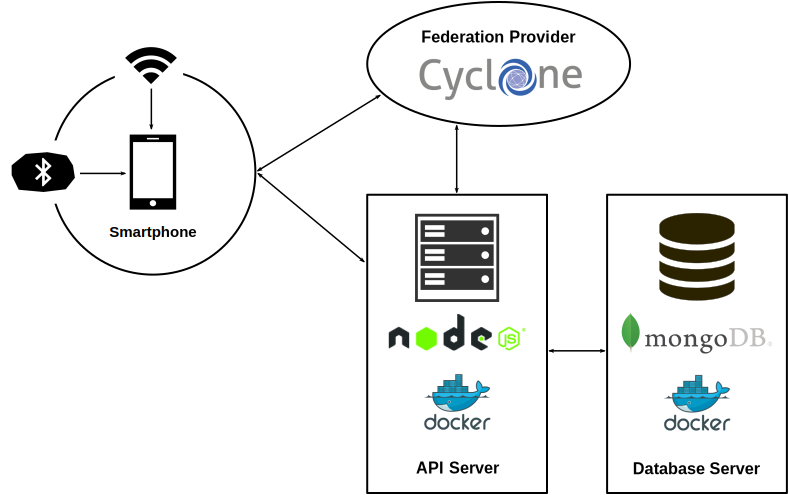
\includegraphics[width=\textwidth]{system-overview}\\
    All components of our envisioned system working together.
    \label{fig:system-overview}
\end{center}

To sum it up, the idea was to gather position information aligned to the user's preferences locally on the smartphone, preform some processing steps on it, contact our backend for which authentication via the CYCLONE Federation Provider is needed and after that create, read, update or delete information (CRUD principle\footnote{\url{https://en.wikipedia.org/wiki/Create,_read,_update_and_delete}}) in the backend and therefore in the database.


\vspace{0.5cm}

\section{API Considerations}

We had to decide on which paradigm our API should be based on. With the client-server and stateless nature of our envisioned system setup in combination with the just mentioned approach of relying on HTTP verbs such as POST, GET, PUT and DELETE for the CRUD operations, the decision to go for a RESTful API was quite clear (\cite{fielding2000architectural}, chapter 5).

Furthermore a widely supported and light-weight format for interchanging data between clients and backend was needed, and it was decided to use JSON\footnote{\url{http://json.org/}}. This also played nicely together with our requirement to implement the API server in Node.JS\footnote{\url{https://nodejs.org/en/}}, using the Express web framework\footnote{\url{http://expressjs.com/}} which provided us a convenient way to define the RESTful resources of our API.


\vspace{0.5cm}

\section{Workload Split Between Clients and Backend}

Our system setup required a certain workload split between the two logical parties, the client side and the backend side. The modification of data on backend side was designed to be very transparent to clients but still some values submitted on the endpoints needed preprocessing to be done on mobile application side.

The general idea is to have the clients handle all direct user interaction with the service in a consistent, user-friendly manner. The other important task on client side is to gather the position information of the requesting user and performing priorization logic on all available information. This was needed to deliver only the most important position to backend where it would replace the old value. The following priorization order was chosen:
\begin{center}
    
\includegraphics[width=0.75\textwidth]{position-priorization-order}\\
    Position priorization order: pin-pointed better than Bluetooth better than WiFi position.
    \label{fig:position-priorization}
\end{center}

On backend side received data would than be sanitized, error and security checked and processed in its according request handler function. Therefore backend would handle everything concerning long term user state management, data persistence and API response aggregation.


\vspace{0.5cm}

\section{Authentication and Session Management}
\label{concept-authentication}

The CYCLONE Federation Provider provided us with the ability to integrate a well-tested user authentication method with only little effort into our service. CYCLONE is based on the JBoss Keycloak\footnote{\url{http://keycloak.jboss.org/}} project which in turn is based on the OpenID Connect standard\footnote{\url{https://openid.net/connect/}}, OAuth 2.0\footnote{\url{http://oauth.net/2/}}, JSON Web Token\footnote{\url{https://jwt.io/}} and SAML 2.0. In the following a short overview of the involved technologies will be given.

The OpenID Connect standard provides two important functionalities in focus of our project. The first one is the addition of an identity layer on top of the OAuth 2.0 Authorization Framework that enables developers to reliable verify what person is using the authenticated service, no matter the used client, be it web or native applications. OpenID Connect does this without the need to maintain password storages on developers' side. Specifically, the CYCLONE Federation Provider uses the Authorization Code Flow\footnote{\url{https://openid.net/specs/openid-connect-core-1_0.html\#CodeFlowAuth}} of the OpenID Connect standard. The other feature OpenID Connect brings into the project is that it already is built as a RESTful HTTP API based on JSON as the transport format and therefore perfectly integrated into the implementation and also provides the functionality to extend the specification in order to, for example, encrypt the transported identity data.

The OAuth 2.0 Authorization Framework is an IETF RFC \cite{hardt2012oauth} which introduces an abstraction layer, the authentication layer, in distributed web application environments. Therefore the standard is designed for the HTTP protocol and does not specify other protocols. OAuth 2.0 provides the ability to differentiate between resource owners (e.g. end users on a service, the resource server) and requesting third parties that need access to some or all resources of the resource owner. Third parties will never need to be authenticated by the resource owner's own credentials but will instead request an access token issued for specific scope, access duration and further attributes from an authorization server. This flow lets the resource owner be in full control of all allowed access requests from third parties, enabling her/him to eventually revoke granted access. Furthermore the attack vector on each involved participants in the service is isolated by separating all authorizations via the access tokens. An extensive threat model analysis on OAuth 2.0 can be found in \cite{lodderstedt2013oauth}.

JWTs (pronouned: \enquote{jots}) are another IETF RFC \cite{bradley2015json} standardizing the transfer of a set of claims as a JSON object in a compact and URL-safe manner. The standard defines three parts of an JWT with the first one being the algorithm and token part, the second being the payload and the third used to verfiy the transported JWT. Encoding and concatenating these fields with dots yields the mentioned URL-safe representation predestined to be transported in HTTP Authorization headers or URI query parameters.

This authentication environment helped us to achieve multiple goals in our implementation. First of all users were able to authenticate via their university account as it is part of the edugain collaboration for which CYCLONE acts as an federation provider. Therefore we had a single-sign-on mechanism available by simply integrating CYCLONE. The other major advantage was that we never saw the user's credentials used to authenticate. We were able to rely on the well-tested user authentication code base provided implicitely through the layered mechanisms the CYCLONE Federation Provider contained.


\vspace{0.5cm}

\section{Database Design}

Part of the template we received at the beginning of the project from our supervisors at the SNET department was the integration of a MongoDB\footnote{\url{https://www.mongodb.org/}} as the database for our service. The communication with the database was not done directly via the officially supported Node.JS MongoDB drivers but instead via another layer inbetween, an object mapping library called Mongoose\footnote{\url{http://mongoosejs.com/}}.

MongoDB is a representative of the class of the NoSQL databases. These kind of databases reject the traditional database approach of laying out the whole data landscape in a relational, table-based fashion prior to implementing an architecture. In the class of NoSQL databases again multiple different data models are used, including columns, documents, key-value stores, graphs or multi-modal databases. MongoDB itself is a document-oriented data store based on the \enquote{Binary JSON} (BSON, pronouned \enquote{bison}) data format.

The NoSQL schema provides multiple features favourable for distributed, scalable environments such as big web applications are. NoSQL databases are generally simpler in design, are able to scale horizontally through sharding and provide greater operation speed in some settings. Also MongoDB incorporates a replication mechanism for high availability in which sets of at least two representations of data exist, one being the primary, the other ones being secondary replicas. In case of a failure of the primary replica, the remaining members perform a leader election in order to retain availability.

In our case we defined models consistent to the representation of data in our architecture. The models included an \texttt{user}, a \texttt{location}, a \texttt{companionrequest} and a \texttt{hotspot} model which in turn got converted into MongoDB collections. Via Mongoose we were able to perform operations on these collections by invoking methods on such a specified model. Further discussion of our model structure will be given in chapter \ref{mongodb-models}.

Of course this setup did not only provide advantages but also yielded quite a lot of headaches during the project. We will be reviewing our issues with MongoDB, or more specifically Mongoose, in our chapter about the evaluation.

\chapter{Implementation}
\label{cha:implementation}


\section{Backend}

\subsection{Architecture}

In this section we will focus on the architecture and our decisions on backend side and its communication. We built a RESTful API which allows clients to communicate with the backend via the JSON format. The figure \ref{fig:system-overview} shows what the architecture consisted of. We had two different client applications which were communicating with the backend and a federation provider,further backend specific information about the federation provider will follow in chapter \ref{federation-provider}. The backend persisted the data into a mongoDB database. The SNET department provided us a virtual machine at the address \url{http://piazza.snet.tu-berlin.de}, where we could setup our environment.

We developed the backend with Node.JS\footnote{\url{https://nodejs.org/en/}} with the purpose that the SNET department could use or integrate it later into other projects which are mostly written in Node.JS. For our web application we used the Express web framework which influenced us in the structure of how our application is built. Our file structure consisted of five main directories:
\begin{itemize}
  \item \textbf{Controllers} are the specific implementation for an API endpoint request.
  \item \textbf{Routes} link an endpoint to a controller.
  \item \textbf{Models} are schemas for the presistent data in the database.
  \item \textbf{Middleware} takes care of our authentication.
  \item \textbf{Tests} are provided for some of the important controllers.
\end{itemize}

\subsection{Controllers}

We designed four controllers which are also part of our API endpoints to handle all requests to our API. \texttt{companionrequests} handles the creation and modification of a companion request. This means that a user wants to add a colleague to her/his friends list and she/he asks her/his friend for permission. If she/he accepts it, both parties are added to each others friends list. If she/he denies it, the requesting user will be notified about the changed status. The controller \texttt{hotspot} gives back all information about the defined hotspots like mensa or library. This includes GPS coordinates, companyUUID, major and minor of the Estimote Bluetooth Beacons contained in the area. For retrieving or modifying user specific information like her/his location, groups and settings the \texttt{users} controller is the handler for these kind of requests. The last controller is the \texttt{login} controller which on successful login returns some information about the logged in user.

\subsection{Routes}

Routes specifies a specific endpoint for a defined URI\footnote{URI=Uniform Resource Identifier}. Our routes link mostly with the same name to the controllers which we defined above. Since we have an RESTful API the expressjs framework also allows us to define GET,POST,PUT and UPDATE functionality. All endpoints are secured via our middleware which we will describe in section \ref{backend-middleware}.

\subsection{Models}
\label{mongodb-models}

Mongoose\footnote{\url{http://mongoosejs.com/}} is a powerful plugin for nodejs which allows us to have an easier connection to the mongoDB database. For this we have to define schema's for our models. So we definded four schemas companionrequest, hotspot, location and user. But not every information have to be an extra collection in the mongoDB. We definded subdocuments for those information which dont need an extra collection. For example the beacons are always in a hotspot so there is no need for an extra collection.

%define models

\subsection{Middleware}
\label{backend-middleware}

The middleware is provided by the cyclone projekt which handels the authentication and session management to the federation provider. If the user doesn't exist in our database the authentication middleware will add it with the informations which he gets from the federation provider. This includes the name, email and the ID which is also given from the authentication token of the user. We overloaded this middleware for the test section below. Which allows us to have a valid authentication against the database.

\subsection{Test}

- Server setup\\
- Docker deployment\\
- List of important API endpoints\\
- Tests

\subsection{CYCLONE Federation Provider}
\label{federation-provider}

\begin{center}
    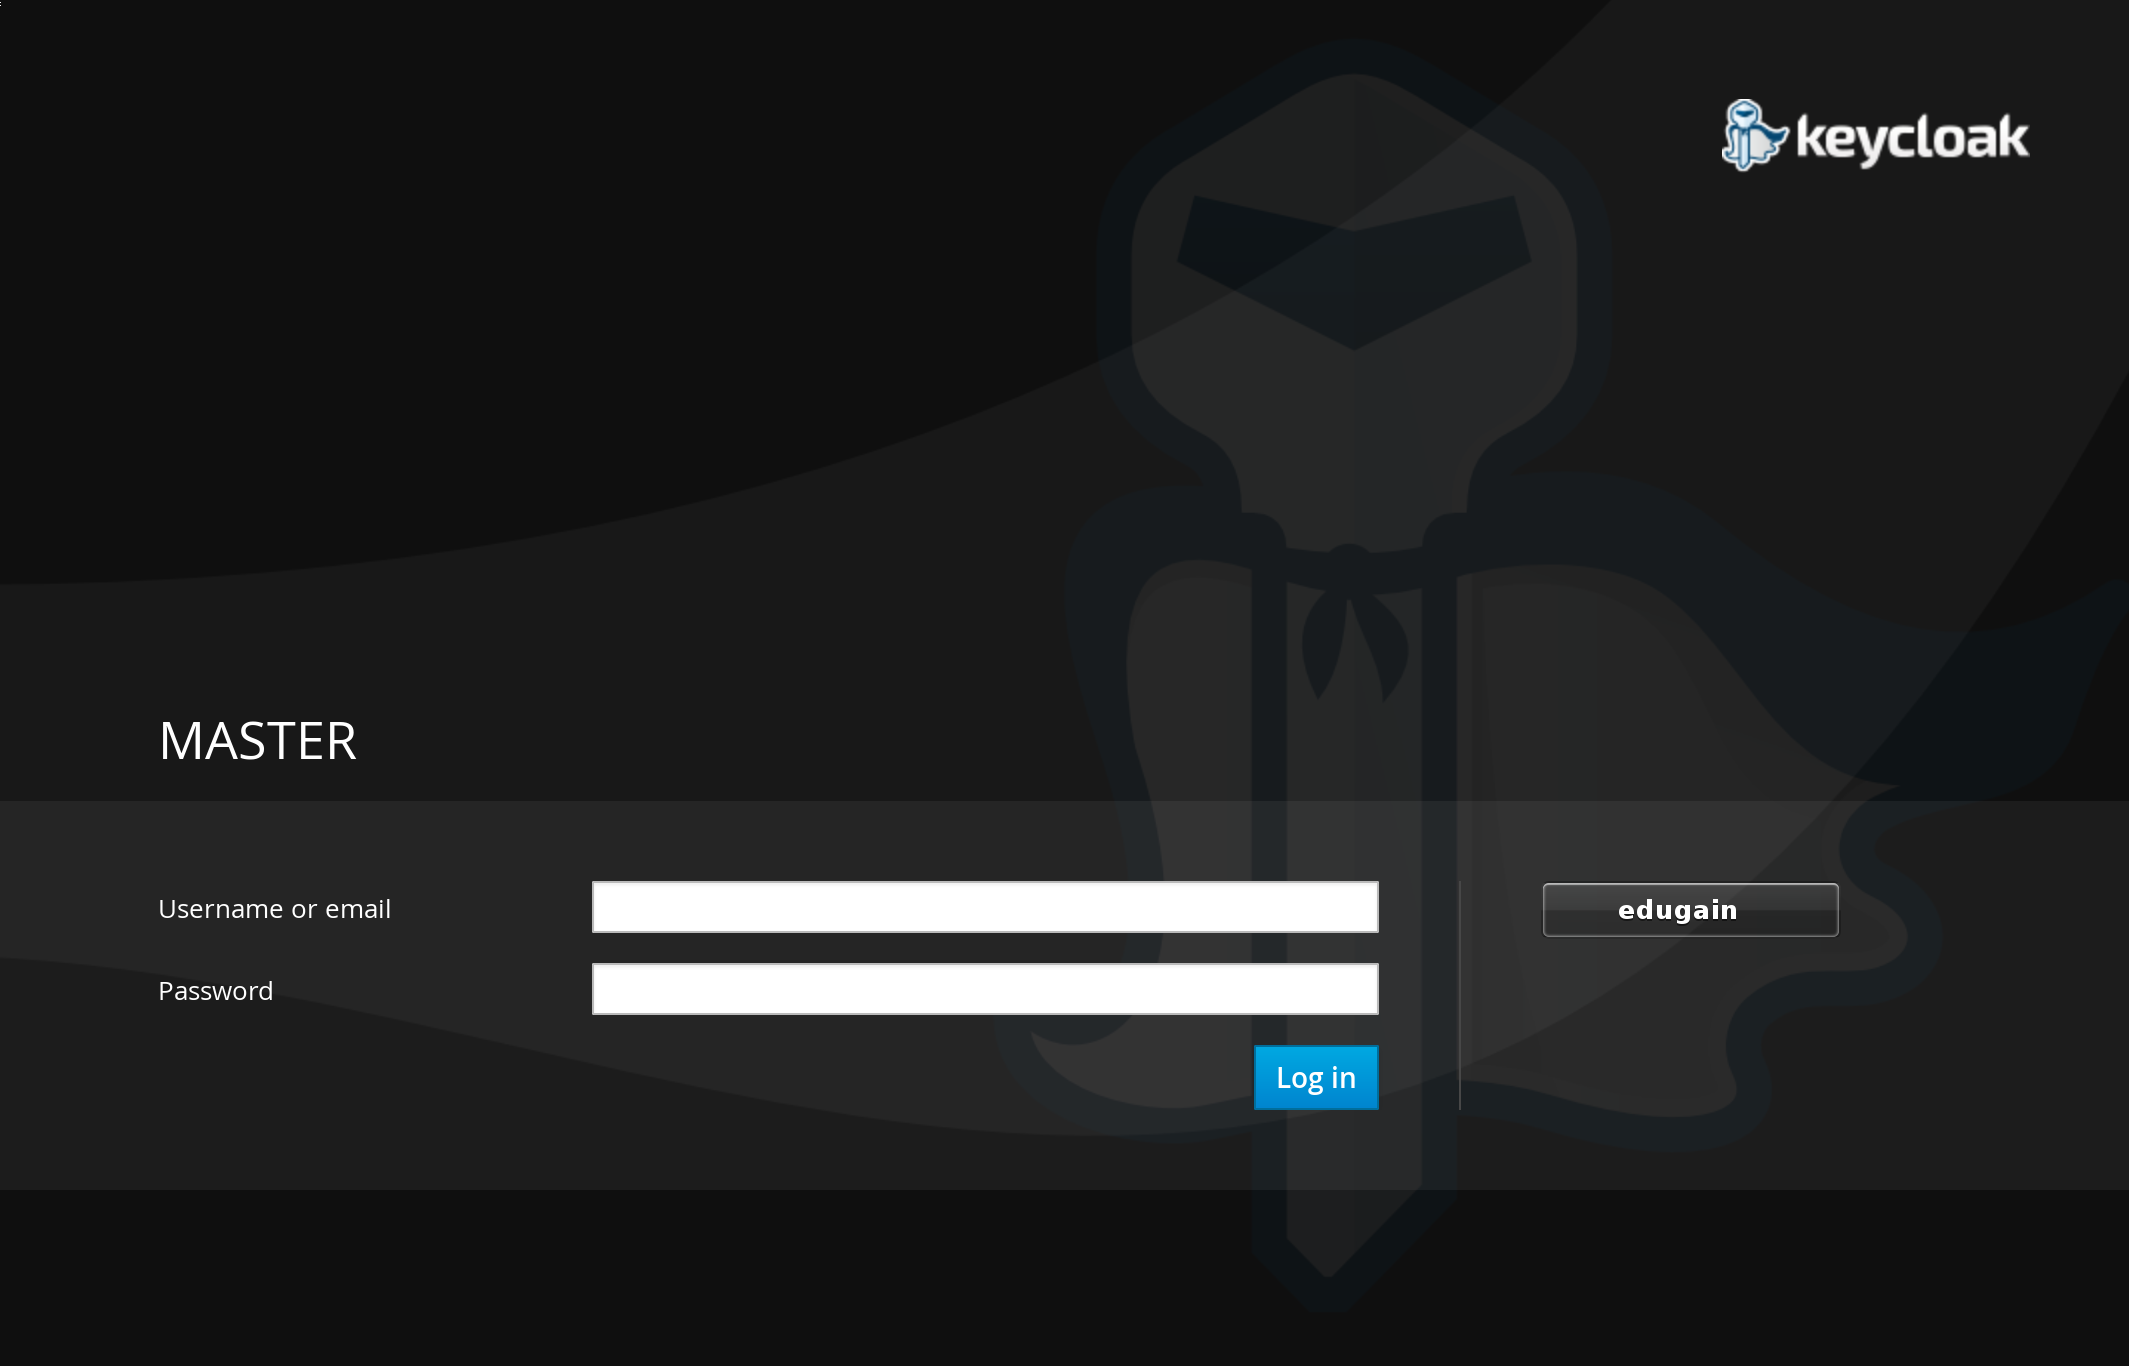
\includegraphics[width=\textwidth]{cyclone-federation-provider-login}\\
    Login screen to CYCLONE Federation Provider.
\end{center}


\vspace{0.5cm}

\section{Android}




\vspace{0.5cm}

\section{iOS}
\subsection{Login}

In order to use the application, the user has to login via Federation Provider, in order to get
a security token which grants access to the application server. \\

The app handles the login process using a UIWebView. The login request will then be redirected
to the Tubit login page ~\ref{fig:login1}, where the user finally can type in Tubit username and password.
If the user credentials are correct, the webview gets redirected to the piazza application server.

If the WebView was able to access the application server successfully, the WebView closes and grants the user access to the application. The WebView can not be bypassed without a successful login via Federation Provider ~\ref{fig:login2}. Each request to the application server reopens the WebView again, if the used security token is invalid or if the user has been logged out.


\begin{figure}
\centering
\begin{minipage}{.5\textwidth}
  \centering
  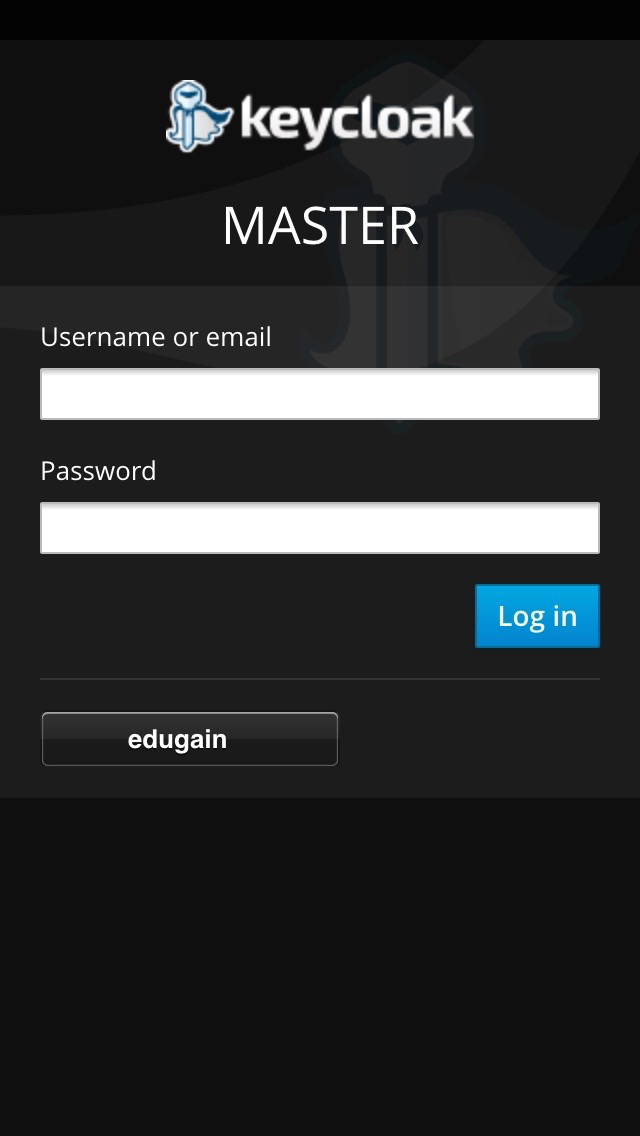
\includegraphics[width=.5\linewidth]{login1}
  \captionof{figure}{Federation Provider}
  \label{fig:login1}
\end{minipage}%
\begin{minipage}{.5\textwidth}
  \centering
  
\includegraphics[width=.5\linewidth]{login2}
  \captionof{figure}{Tubit Login}
  \label{fig:login2}
\end{minipage}
\end{figure}

\subsection{Hotspots/ Buildings}

\begin{figure}
\centering
\begin{minipage}{.5\textwidth}
  \centering
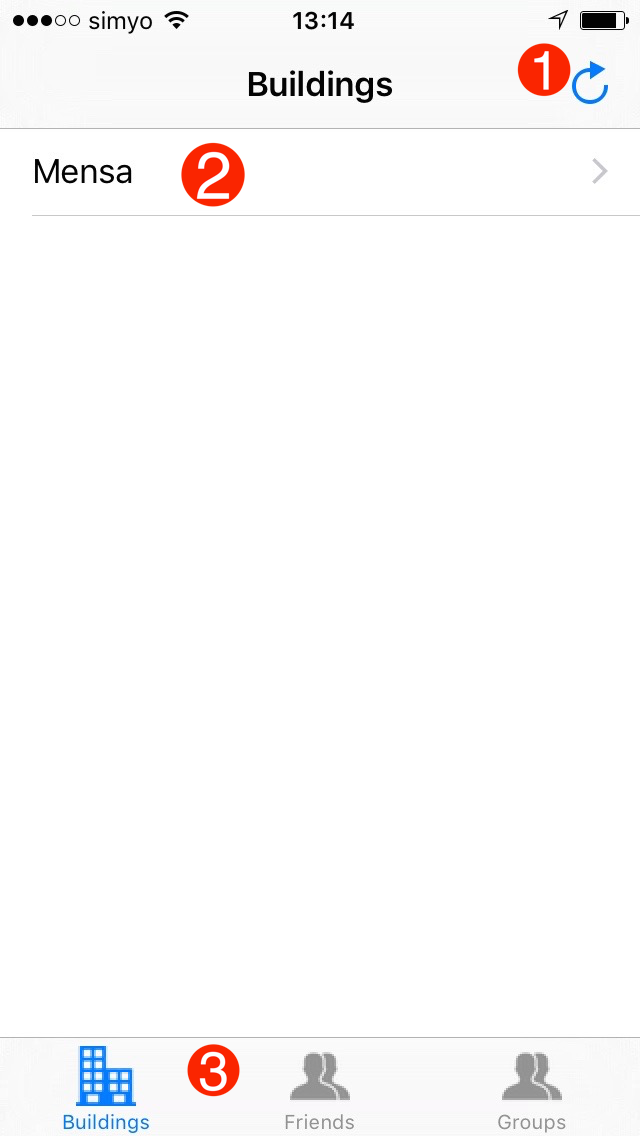
\includegraphics[width=.5\linewidth]{showbuildings}
\caption{TableView with a list of Buildings}
\label{fig:showbuildings}
\end{minipage}
\end{figure}

The Buildings View ~\ref{fig:showbuildings} is the first view the user sees after login. This view enlists all available Hotspots delivered by the Backend.

\begin{enumerate}
  \item The reload button, calls the Backend to get a list of available hotspots. The list contains the hotspots and the available beacon and floor information.
  \item The Tableview lists all available hotspots from the Backend. Each cell contains the name of a Hotspot.
  \item The Application is divided into three contextual distinct parts: Buildings, Friends and Groups. This subdivision is implemented in a UITabBar which is the leading element of the application architecture.
\end{enumerate}

\subsection{Friends}

%%%%%%%%%%%%%%%%%%%%%%%%%%%%%%%
\begin{figure}
\centering
\begin{minipage}{.5\textwidth}
  \centering
  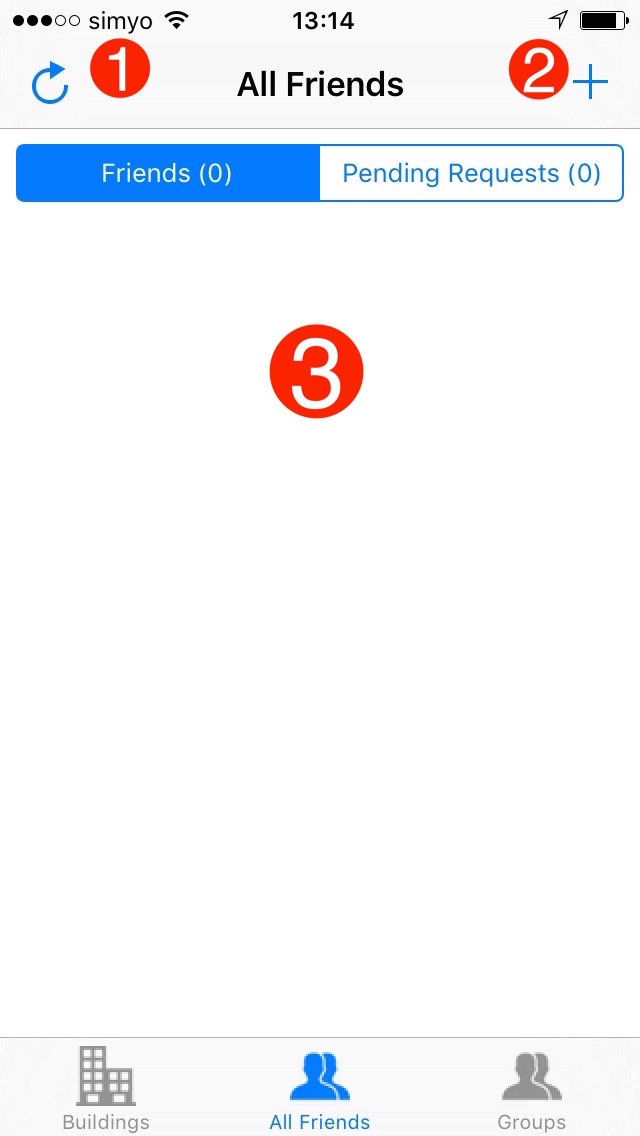
\includegraphics[width=.5\linewidth]{friendlist}
  \captionof{figure}{Available Friends and Open Requests}
  \label{fig:friendlist}
\end{minipage}%
\begin{minipage}{.5\textwidth}
  \centering
  
\includegraphics[width=.5\linewidth]{addfriend}
  \captionof{figure}{Add Friends}
  \label{fig:addfriend}
\end{minipage}
\end{figure}

\begin{figure}
\centering
\begin{minipage}{.5\textwidth}
  \centering
  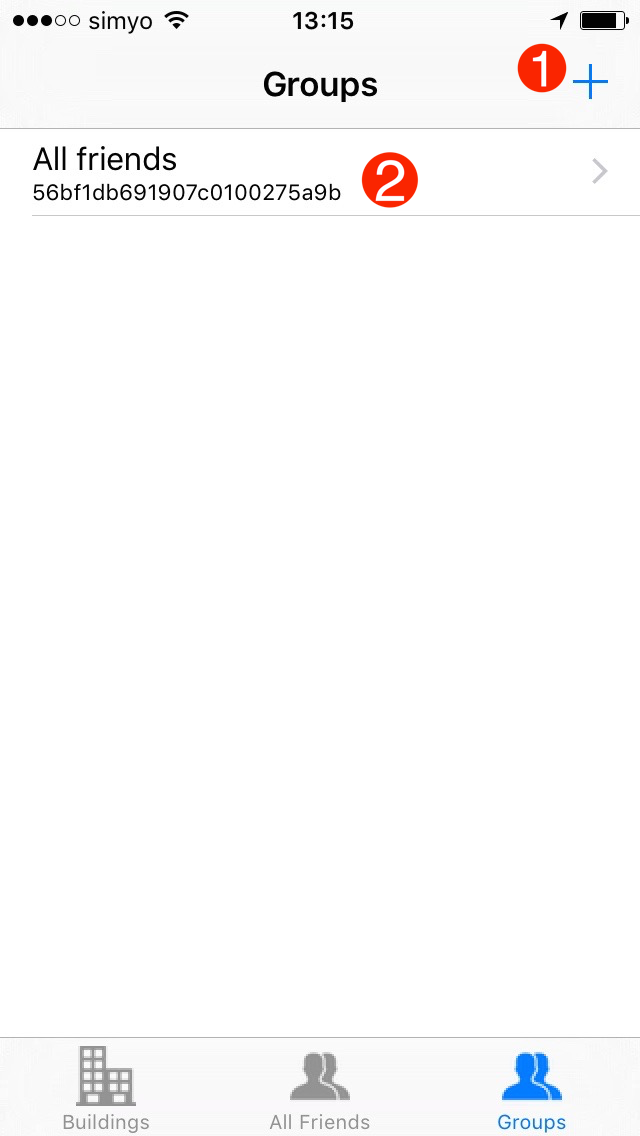
\includegraphics[width=.5\linewidth]{showgroups}
  \captionof{figure}{Available Groups}
  \label{fig:showgroups}
\end{minipage}%
\begin{minipage}{.5\textwidth}
  \centering
  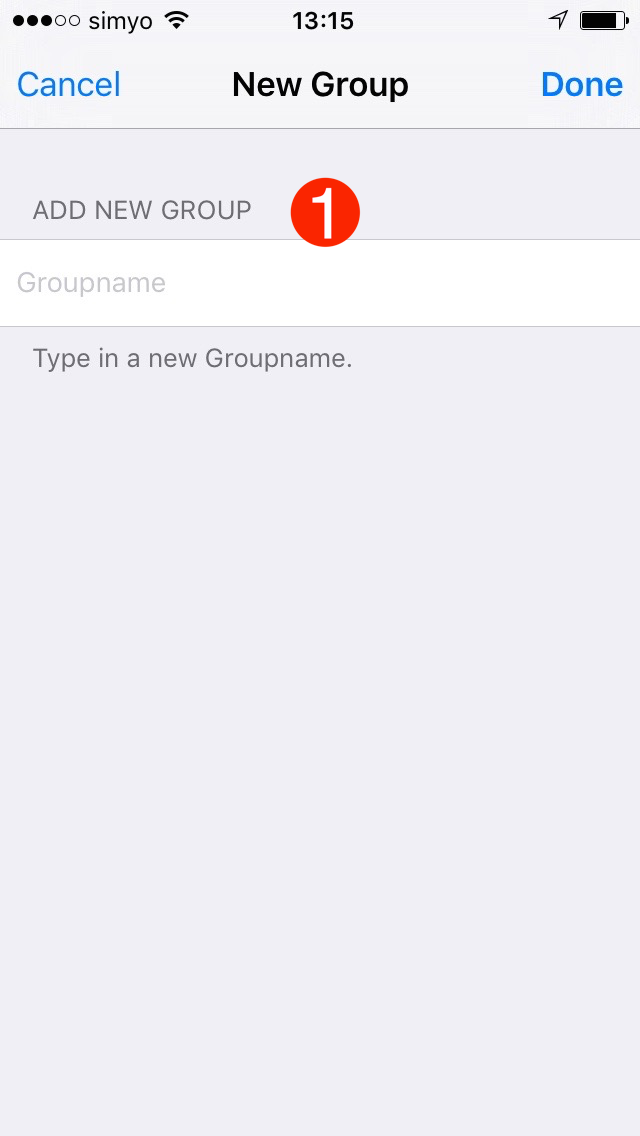
\includegraphics[width=.5\linewidth]{addgroup}
  \captionof{figure}{Add Group}
  \label{fig:addgroup}
\end{minipage}
\end{figure}

\begin{figure}
\centering
\begin{minipage}{.5\textwidth}
  \centering
  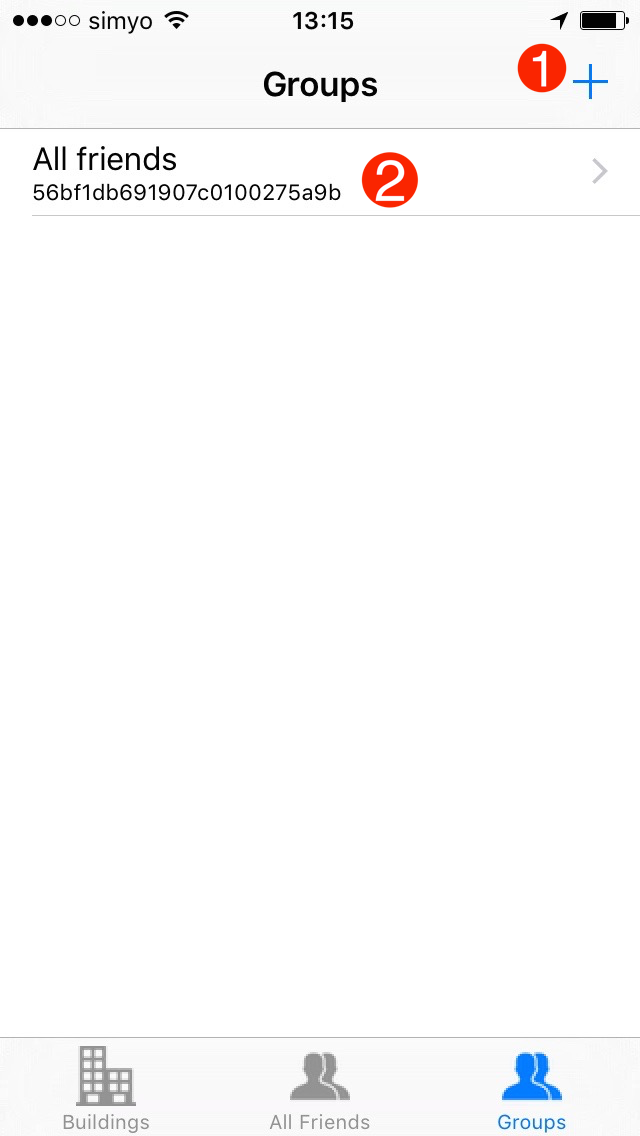
\includegraphics[width=.5\linewidth]{showgroups}
  \captionof{figure}{Available Groups}
  \label{fig:showgroups}
\end{minipage}%
\begin{minipage}{.5\textwidth}
  \centering
  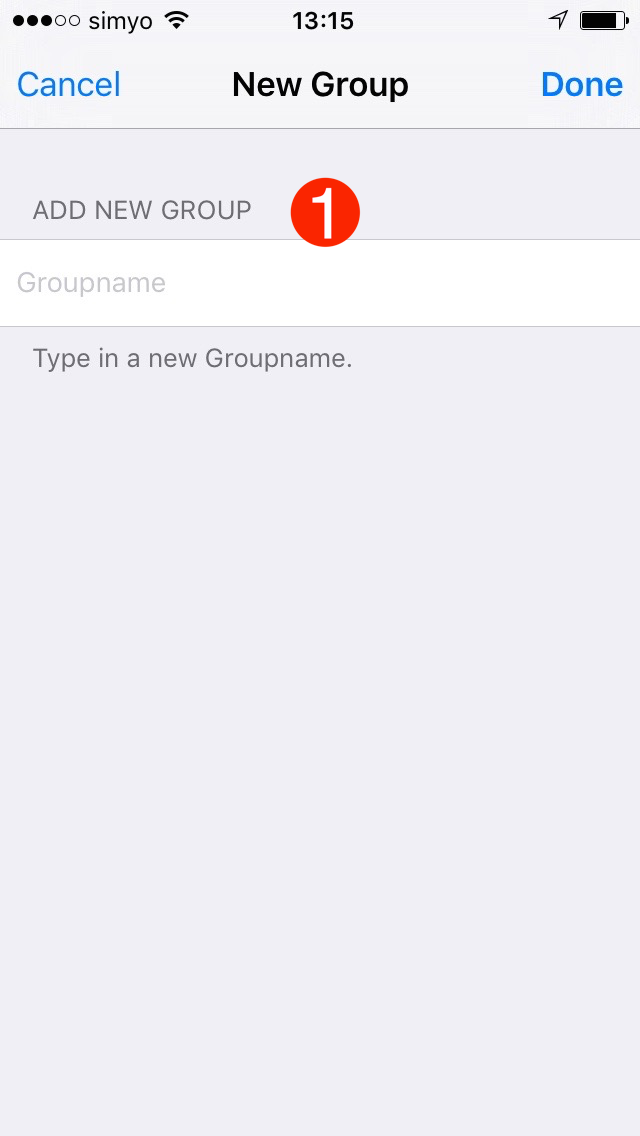
\includegraphics[width=.5\linewidth]{addgroup}
  \captionof{figure}{Add Group}
  \label{fig:addgroup}
\end{minipage}
\end{figure}

\begin{figure}
\centering
\begin{minipage}{.5\textwidth}
  \centering
  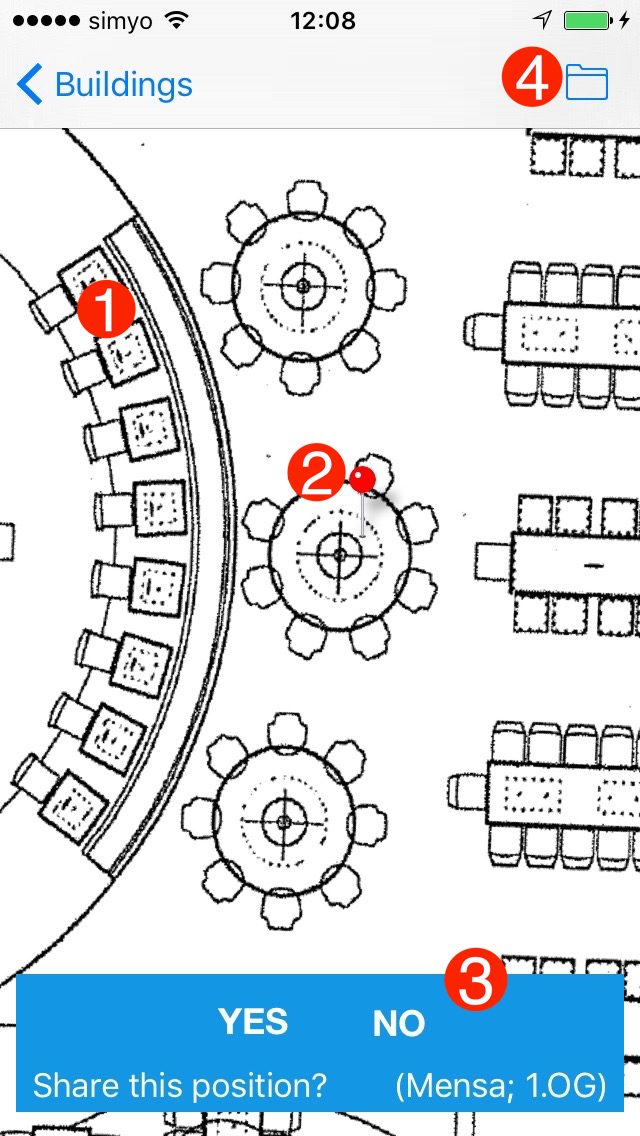
\includegraphics[width=.5\linewidth]{shareposition}
  \captionof{figure}{Share Position Mode}
  \label{fig:shareposition}
\end{minipage}%
\begin{minipage}{.5\textwidth}
  \centering
  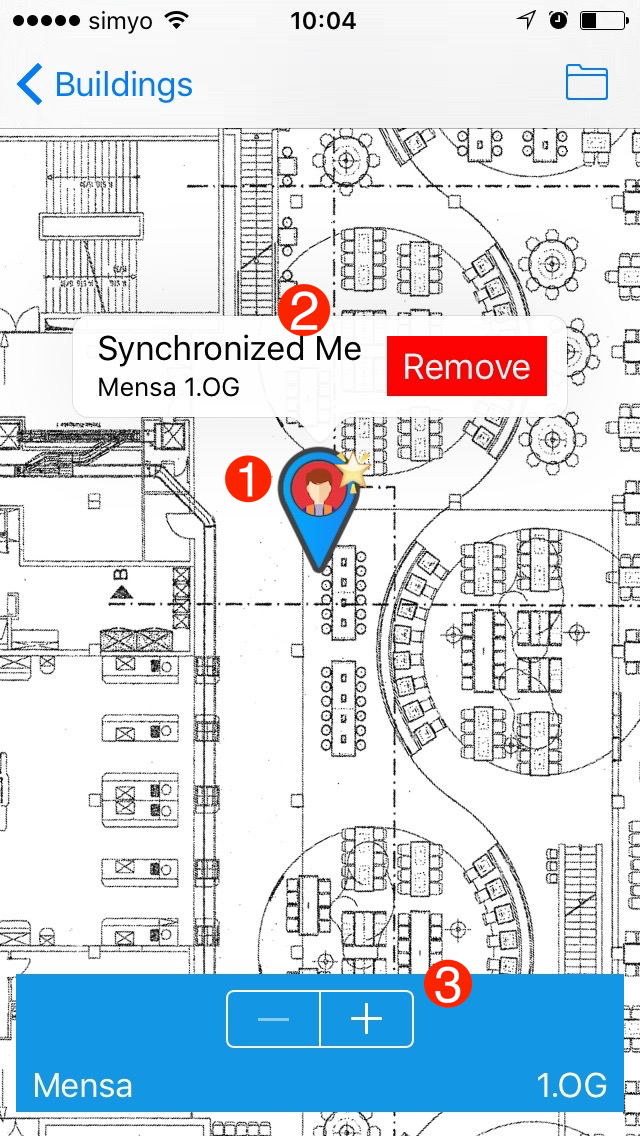
\includegraphics[width=.5\linewidth]{synchronizedme}
  \captionof{figure}{Synchronized Position Mode}
  \label{fig:synchronizedme}
\end{minipage}
\end{figure}

\begin{figure}
\centering
\begin{minipage}{.5\textwidth}
  \centering
  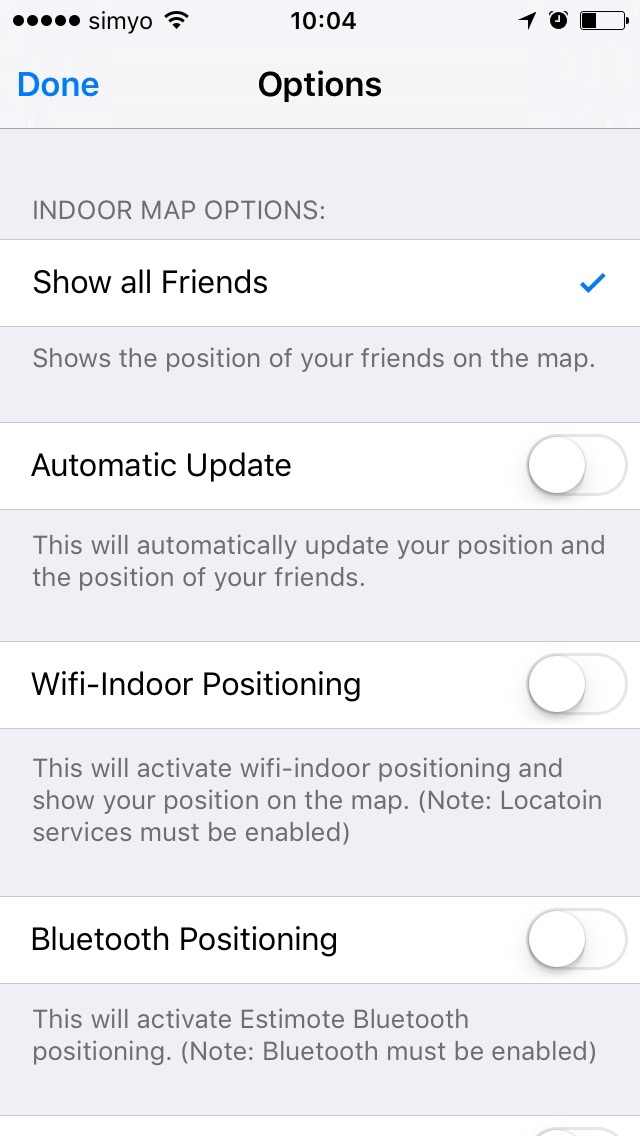
\includegraphics[width=.5\linewidth]{settings1}
  \captionof{figure}{Share Position Mode}
  \label{fig:settings1}
\end{minipage}%
\begin{minipage}{.5\textwidth}
  \centering
  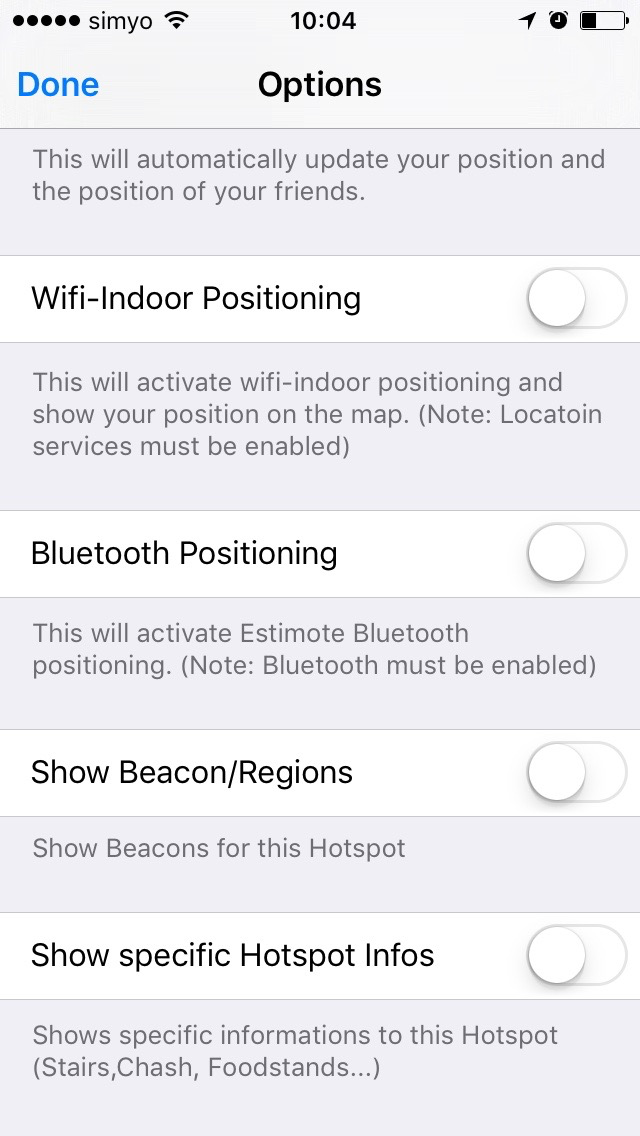
\includegraphics[width=.5\linewidth]{settings2}
  \captionof{figure}{Synchronized Position Mode}
  \label{fig:settings2}
\end{minipage}
\end{figure}



\begin{figure}
\centering
\begin{minipage}{.5\textwidth}
  \centering
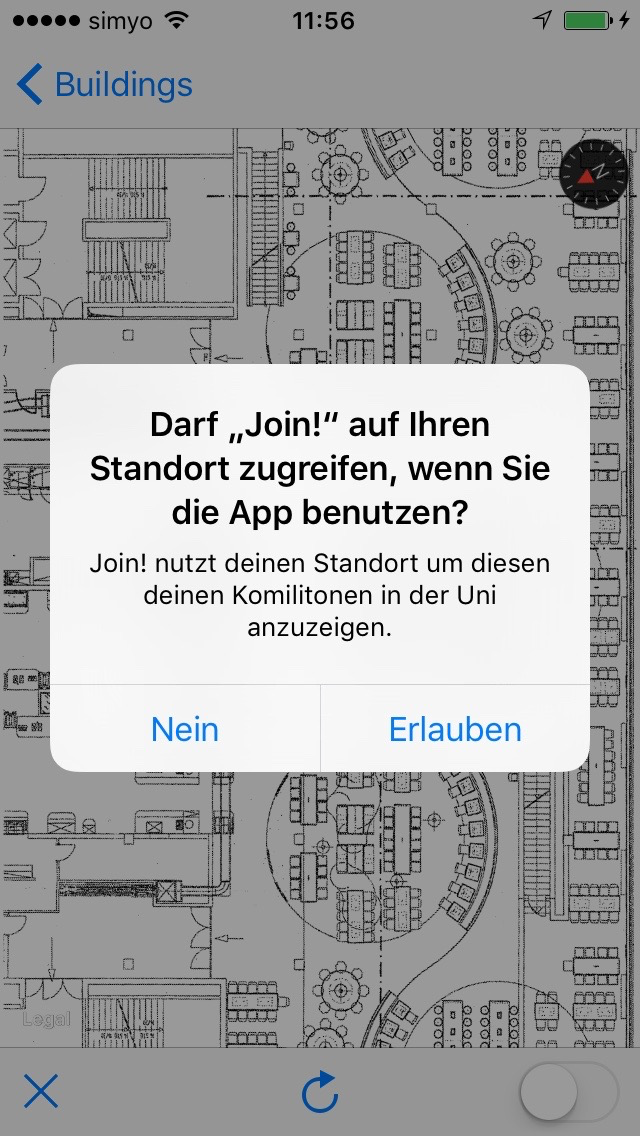
\includegraphics[width=.5\linewidth]{request1}
\caption{TableView with a list of Buildings}
\label{fig:request1}
\end{minipage}
\end{figure}


\begin{figure}
\centering
\begin{minipage}{.5\textwidth}
  \centering
  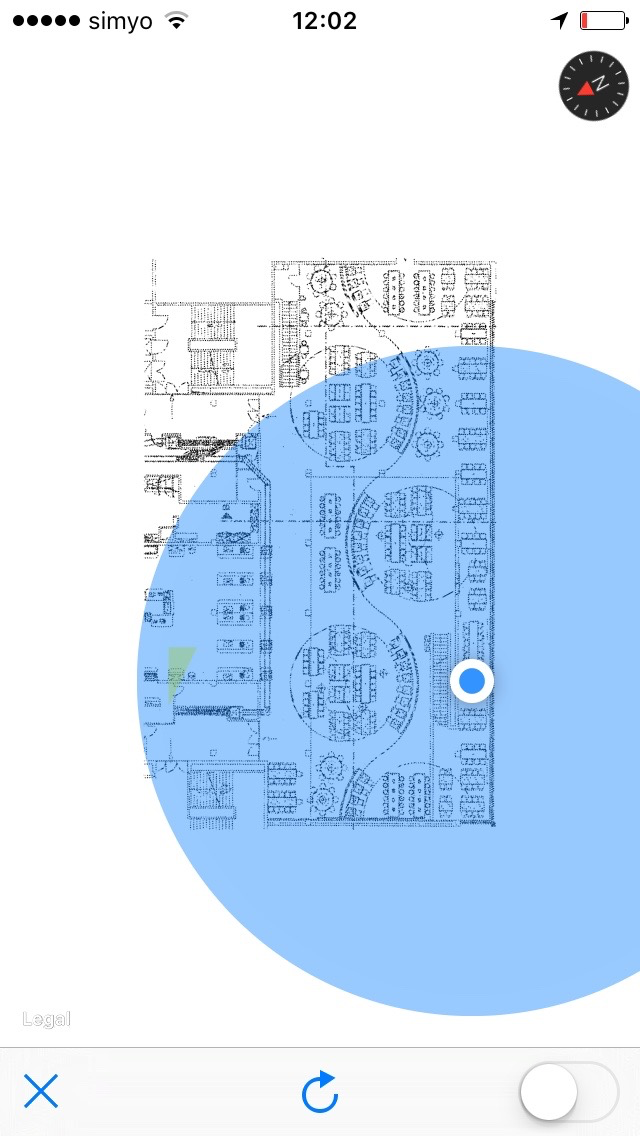
\includegraphics[width=.5\linewidth]{cllocationframework1}
  \captionof{figure}{Share Position Mode}
  \label{fig:cllocationframework1}
\end{minipage}%
\begin{minipage}{.5\textwidth}
  \centering
  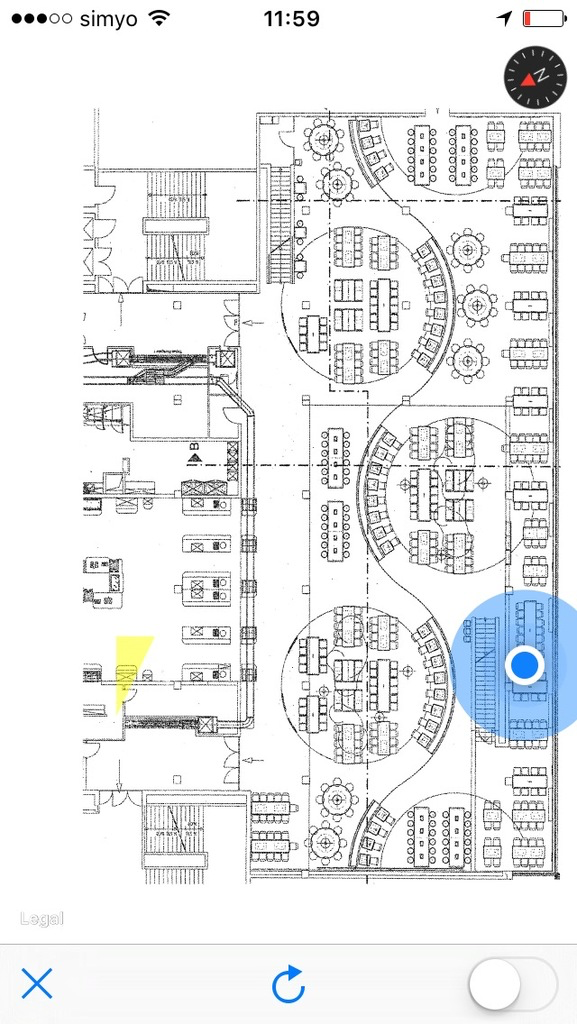
\includegraphics[width=.5\linewidth]{cllocationframework2}
  \captionof{figure}{Synchronized Position Mode}
  \label{fig:cllocationframework2}
\end{minipage}
\end{figure}


\begin{figure}
\centering
\begin{minipage}{.5\textwidth}
  \centering
  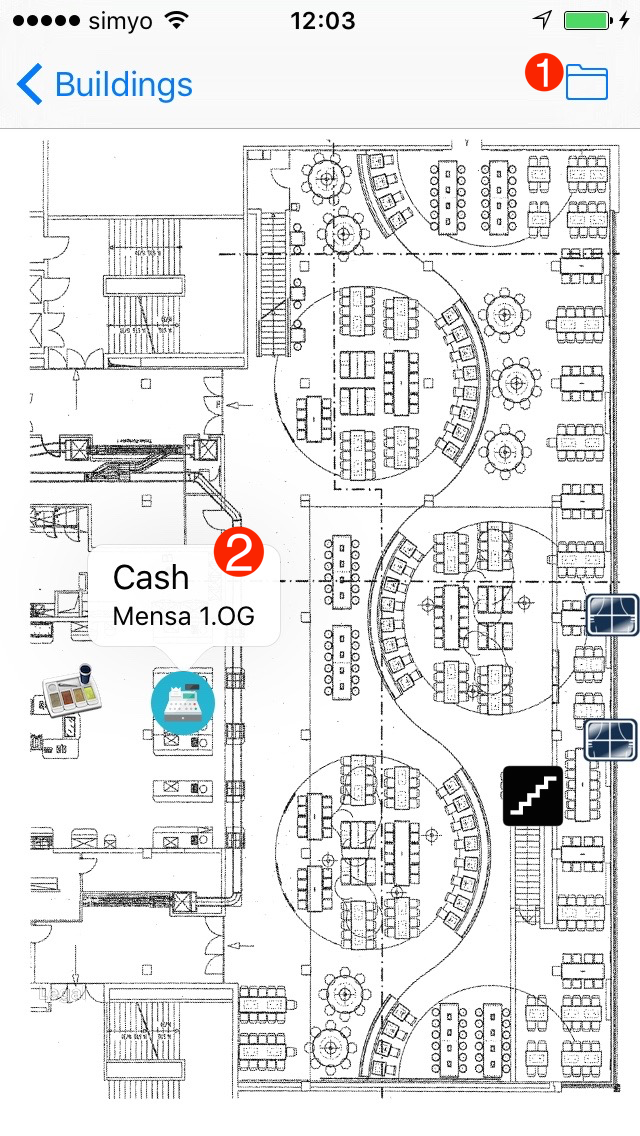
\includegraphics[width=.5\linewidth]{additionalinfo}
  \captionof{figure}{Share Position Mode}
  \label{fig:additionalinfo}
\end{minipage}%
\begin{minipage}{.5\textwidth}
  \centering
  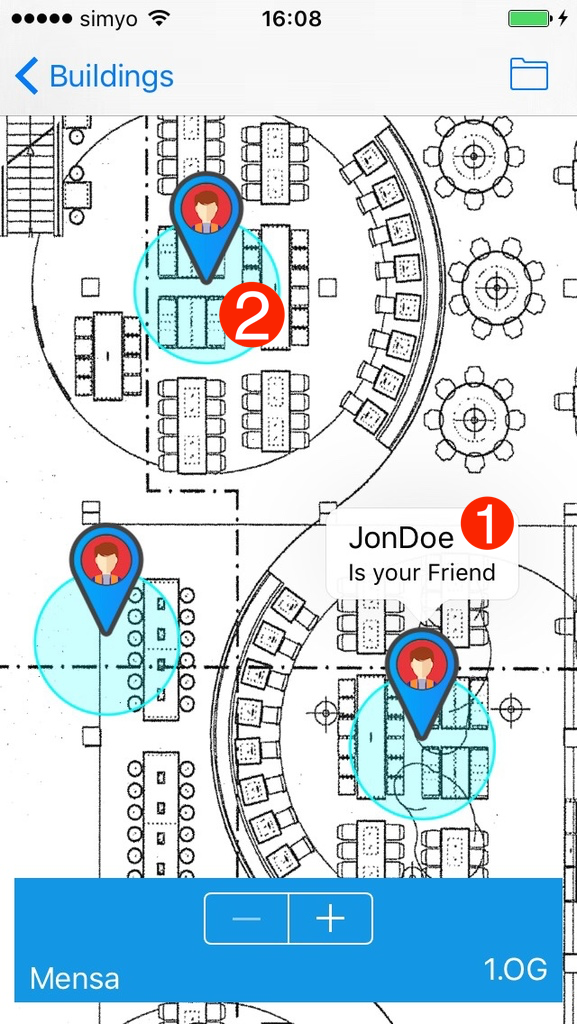
\includegraphics[width=.5\linewidth]{showfriends}
  \captionof{figure}{Synchronized Position Mode}
  \label{fig:showfriends}
\end{minipage}
\end{figure}

\begin{figure}
\centering
\begin{minipage}{.5\textwidth}
  \centering
  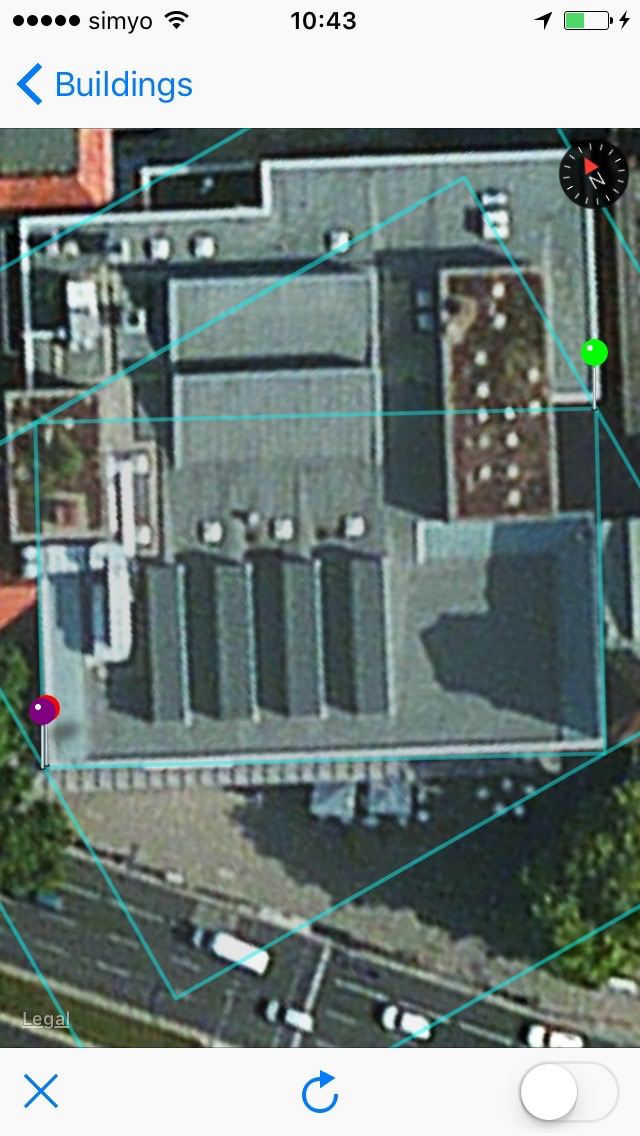
\includegraphics[width=.5\linewidth]{map1}
  \captionof{figure}{Share Position Mode}
  \label{fig:map1}
\end{minipage}%
\begin{minipage}{.5\textwidth}
  \centering
  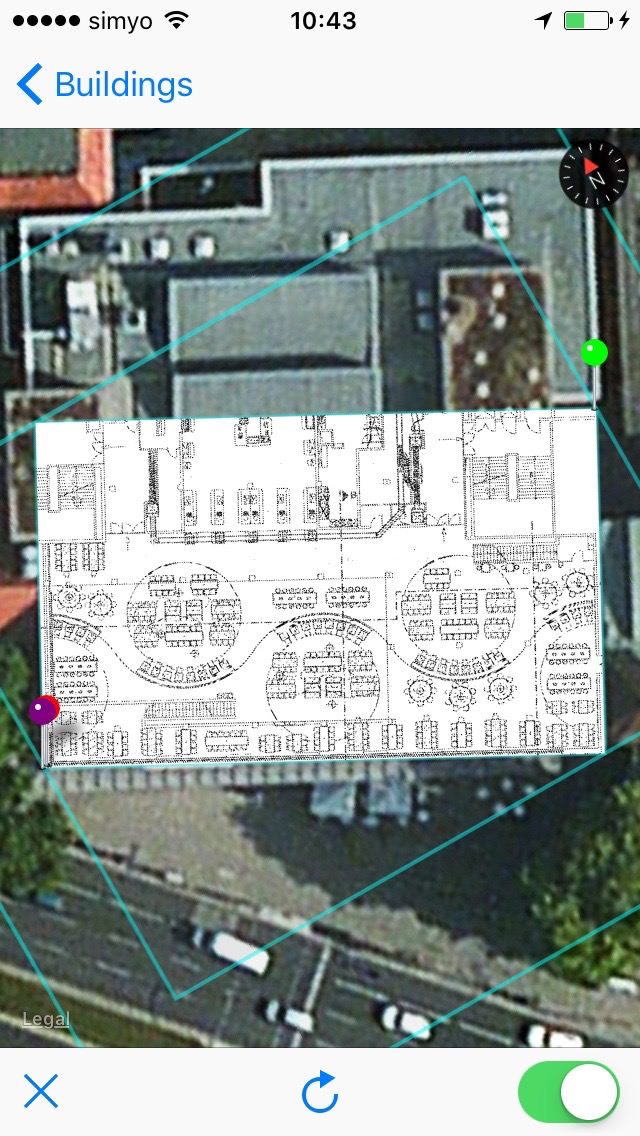
\includegraphics[width=.5\linewidth]{map2}
  \captionof{figure}{Synchronized Position Mode}
  \label{fig:map2}
\end{minipage}
\end{figure}


\begin{enumerate}
  \item The first item
  \begin{enumerate}
    \item Nested item 1
    \item Nested item 2
  \end{enumerate}
  \item The second item
  \item The third etc \ldots
\end{enumerate}




\begin{figure}
\centering

\includegraphics[scale=0.2]{addfriend}
\caption{A prototype of the Add Friend}
\label{fig:addFriendDialog}
\end{figure}

\chapter{Evaluation}
\label{cha:evaluation}

Evaluate:
\begin{itemize}
    \item What does work so far? What does not?
    \item What were the observed issues (see final presentation)?
    \item $\rightarrow$ MSE API, beacons, interplay server with clients, Node.JS, Mongoose (MongoDB), etc.
\end{itemize}
\chapter{Conclusion}
\label{cha:conclusion}

Conclusion:
\begin{itemize}
    \item What did we do, how did it work out?
    \item Mention \enquote{team work issues}?
    \item Future work
\end{itemize}

\hline

\vspace{0.5cm}

\section{Future Work}

%--------------------------------------------------------------
\backmatter

\listoftables
\listoffigures

\setwidesite{}						% Set page to be wider for bibliography

\label{cha:bibliography}
\markboth{Bibliography}{Bibliography}
\addcontentsline{toc}{chapter}{Bibliography}
\printbibliography
%\printbibliography[heading=offline,filter=offline]
%\printbibliography[heading=online,filter=online]

\begin{appendices}

some appendix

\end{appendices}

\end{document}
